% !TEX root = ../main.tex
\documentclass[../main.tex]{subfiles}

\begin{document}
\section{Aufgabenstellung}

\subsection{Hintergrund}

Studierende der Hochschule Luzern werden im Rahmen der Projektmodule
Produktentwicklung 1 und 2 mit der Aufgabe betraut, gemeinsam in einem
interdisziplinären Team eine Lösung für ein spezifisches Problem zu erarbeiten.
Im ersten Teilmodul, PREN 1, dreht sich alles um das Thema Konzeptionierung.
Jedes Team soll verschiedene Lösungsvarianten für die Aufgabenstellung
ausarbeiten und bewerten. Im zweiten Semester, im Folgemodul, wird dieses
Konzept finalisiert und umgesetzt. Am Ende der beiden Semester steht ein
Wettbewerb an, bei dem die verschiedenen Teams mit ihren Lösungen gegeneinander
antreten.

\subsection{Aufgabenstellung}

Es soll ein Fahrzeug entwickelt und gebaut werden, das auf einem mit Weglinien
markierten Wegenetz den optimalen Weg zu einem Ziel finden soll. Dabei können
drei Arten von Ereignissen auftreten, auf die das Fahrzeug reagieren muss. Ziel
ist es, dass das Fahrzeug den Weg autonom und ohne externe Eingriffe findet.
Das Wegenetz ist in Abbildung~\ref{fig:wegenetz} dargestellt:

\begin{figure}[h!]
    \centering
    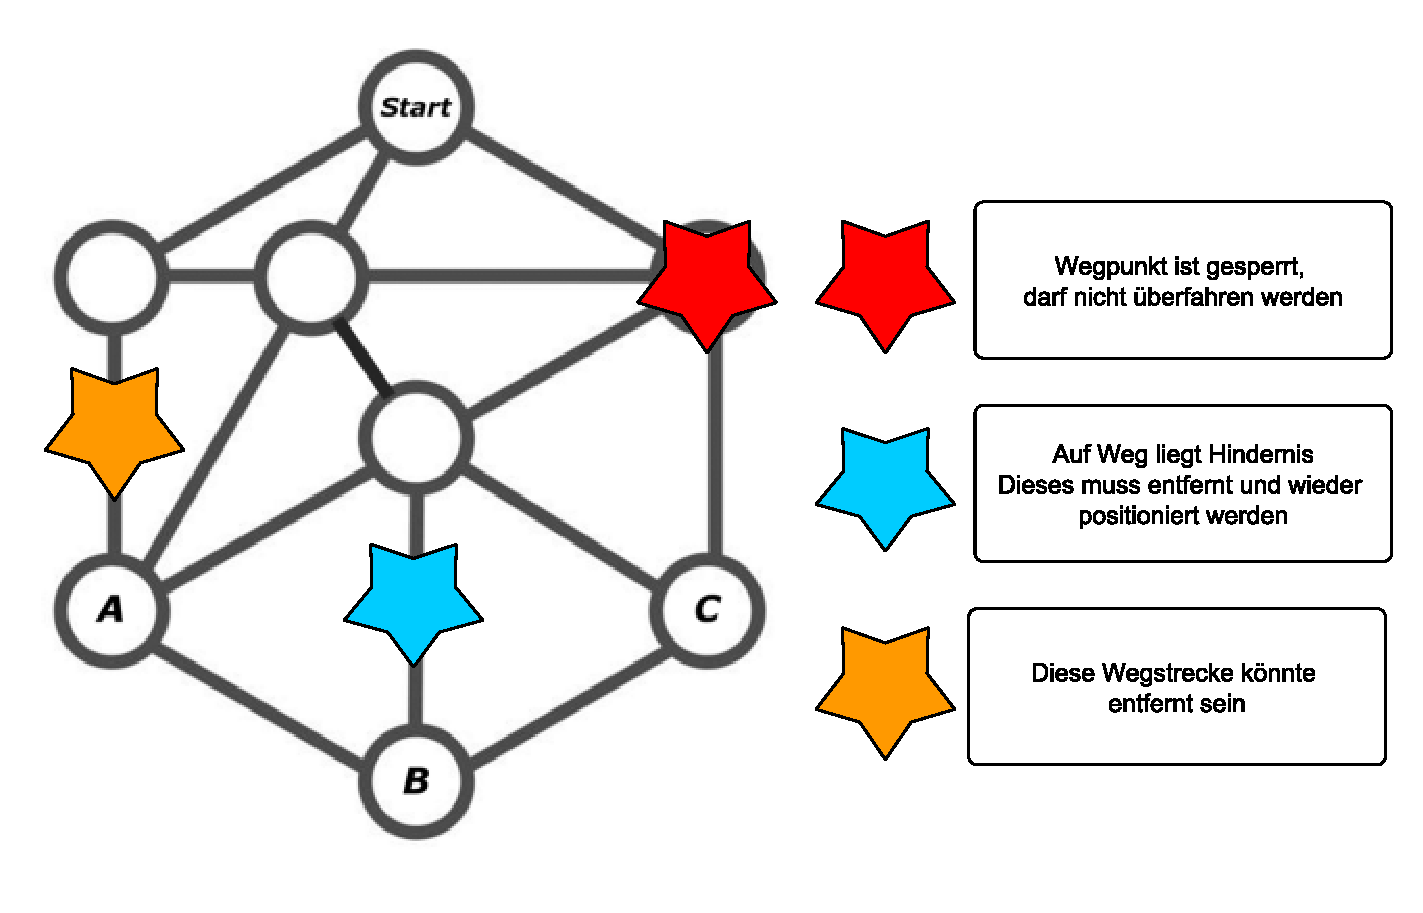
\includegraphics[width=0.6\textwidth]{./resources/Abbildung_Wegenetz.pdf}
    \caption{Wegenetz}
    \label{fig:wegenetz}
\end{figure}

\textbf{Mögliche Ereignisse:}
\begin{itemize}
    \item \textbf{Gesperrter Wegpunkt} (Rot): Punkt darf nicht befahren werden.
    \item \textbf{Hindernis auf der Strecke} (Blau): Das Hindernis muss entfernt werden.
    \item \textbf{Nicht vorhandene Strecke} (Orange): Wird von Schiedsrichtern entfernt.
\end{itemize}

Die entsprechenden Ereignisse auf den Wegen werden vor jedem Start neu
festgelegt und sind im Voraus nicht bekannt. Das gewünschte Ziel wird über
einen physischen Wahlschalter vorgegeben, woraufhin das Fahrzeug automatisch
zum Ziel manövriert. Nach dem Startkommando beginnt die Zeitmessung.

Während der Entwicklung des Fahrzeugs soll besonderes Augenmerk auf die
verwendeten Materialien und deren Lieferwege gelegt werden, um auch der
Nachhaltigkeit Rechnung zu tragen.

\end{document}
